Στην Άσκηση 8, η σχεδίαση μεταφέρθηκε σε ένα πιο ρεαλιστικό επίπεδο υλοποίησης με την προσθήκη του δακτυλίου των ακροδεκτών (Pad Ring), χρησιμοποιώντας τη βιβλιοθήκη \texttt{pads\_SS\_s1v8}. Η επίδραση των pads στα χαρακτηριστικά του κυκλώματος ήταν δραματική, όπως φαίνεται στους Πίνακες 8.1 έως 8.3.

\begin{figure}[H]
    \centering
    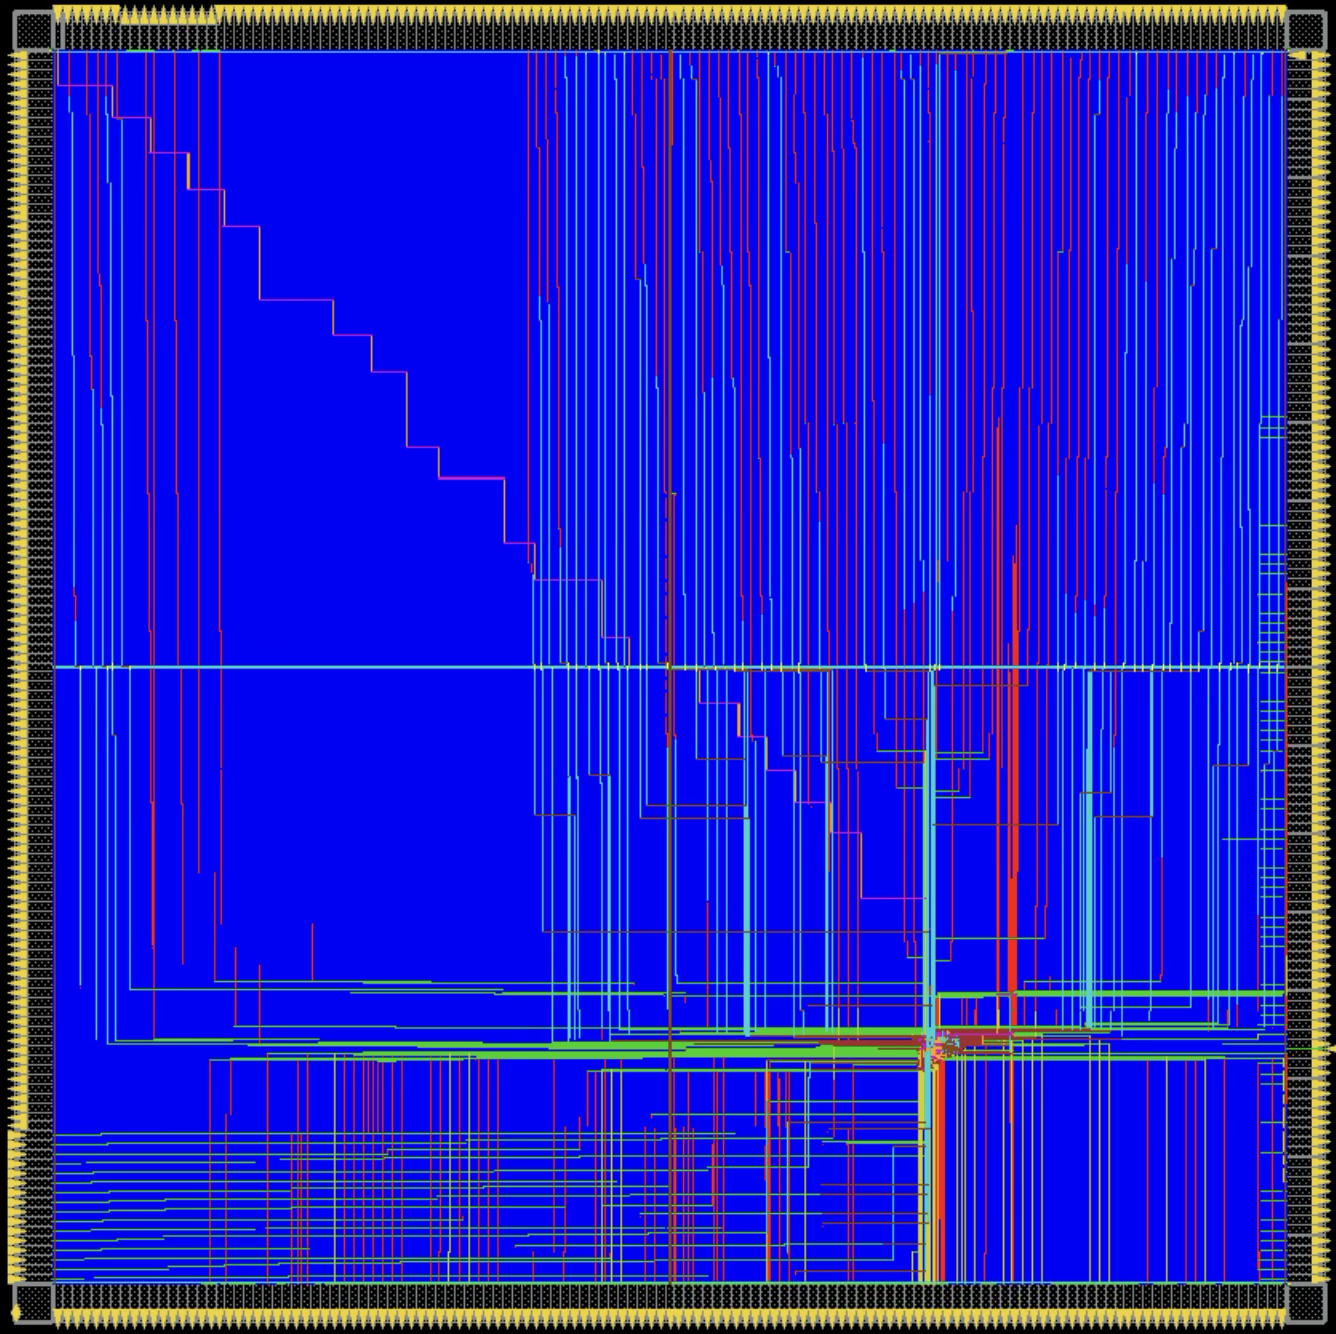
\includegraphics[width=0.8\textwidth]{assets/fig8_1_full_chip.png}
    \caption{Full Chip View}
\end{figure}

Στην απεικόνιση του πλήρους chip, διακρίνονται καθαρά οι κίτρινοι ακροδέκτες (bond pads) στην περιφέρεια, οι οποίοι σχηματίζουν το πλαίσιο επικοινωνίας με το εξωτερικό περιβάλλον. Είναι εμφανής η τεράστια διαφορά μεγέθους μεταξύ του πυρήνα (core logic), που βρίσκεται στο κέντρο, και του συνολικού εμβαδού που καταλαμβάνουν τα pads. Η εικόνα επιβεβαιώνει οπτικά ότι πρόκειται για μια σχεδίαση "Pad Limited", όπου οι διαστάσεις του chip καθορίζονται αποκλειστικά από τον αριθμό των απαιτούμενων ακροδεκτών και όχι από το μέγεθος της λογικής του κυκλώματος.

\begin{figure}[H]
    \centering
    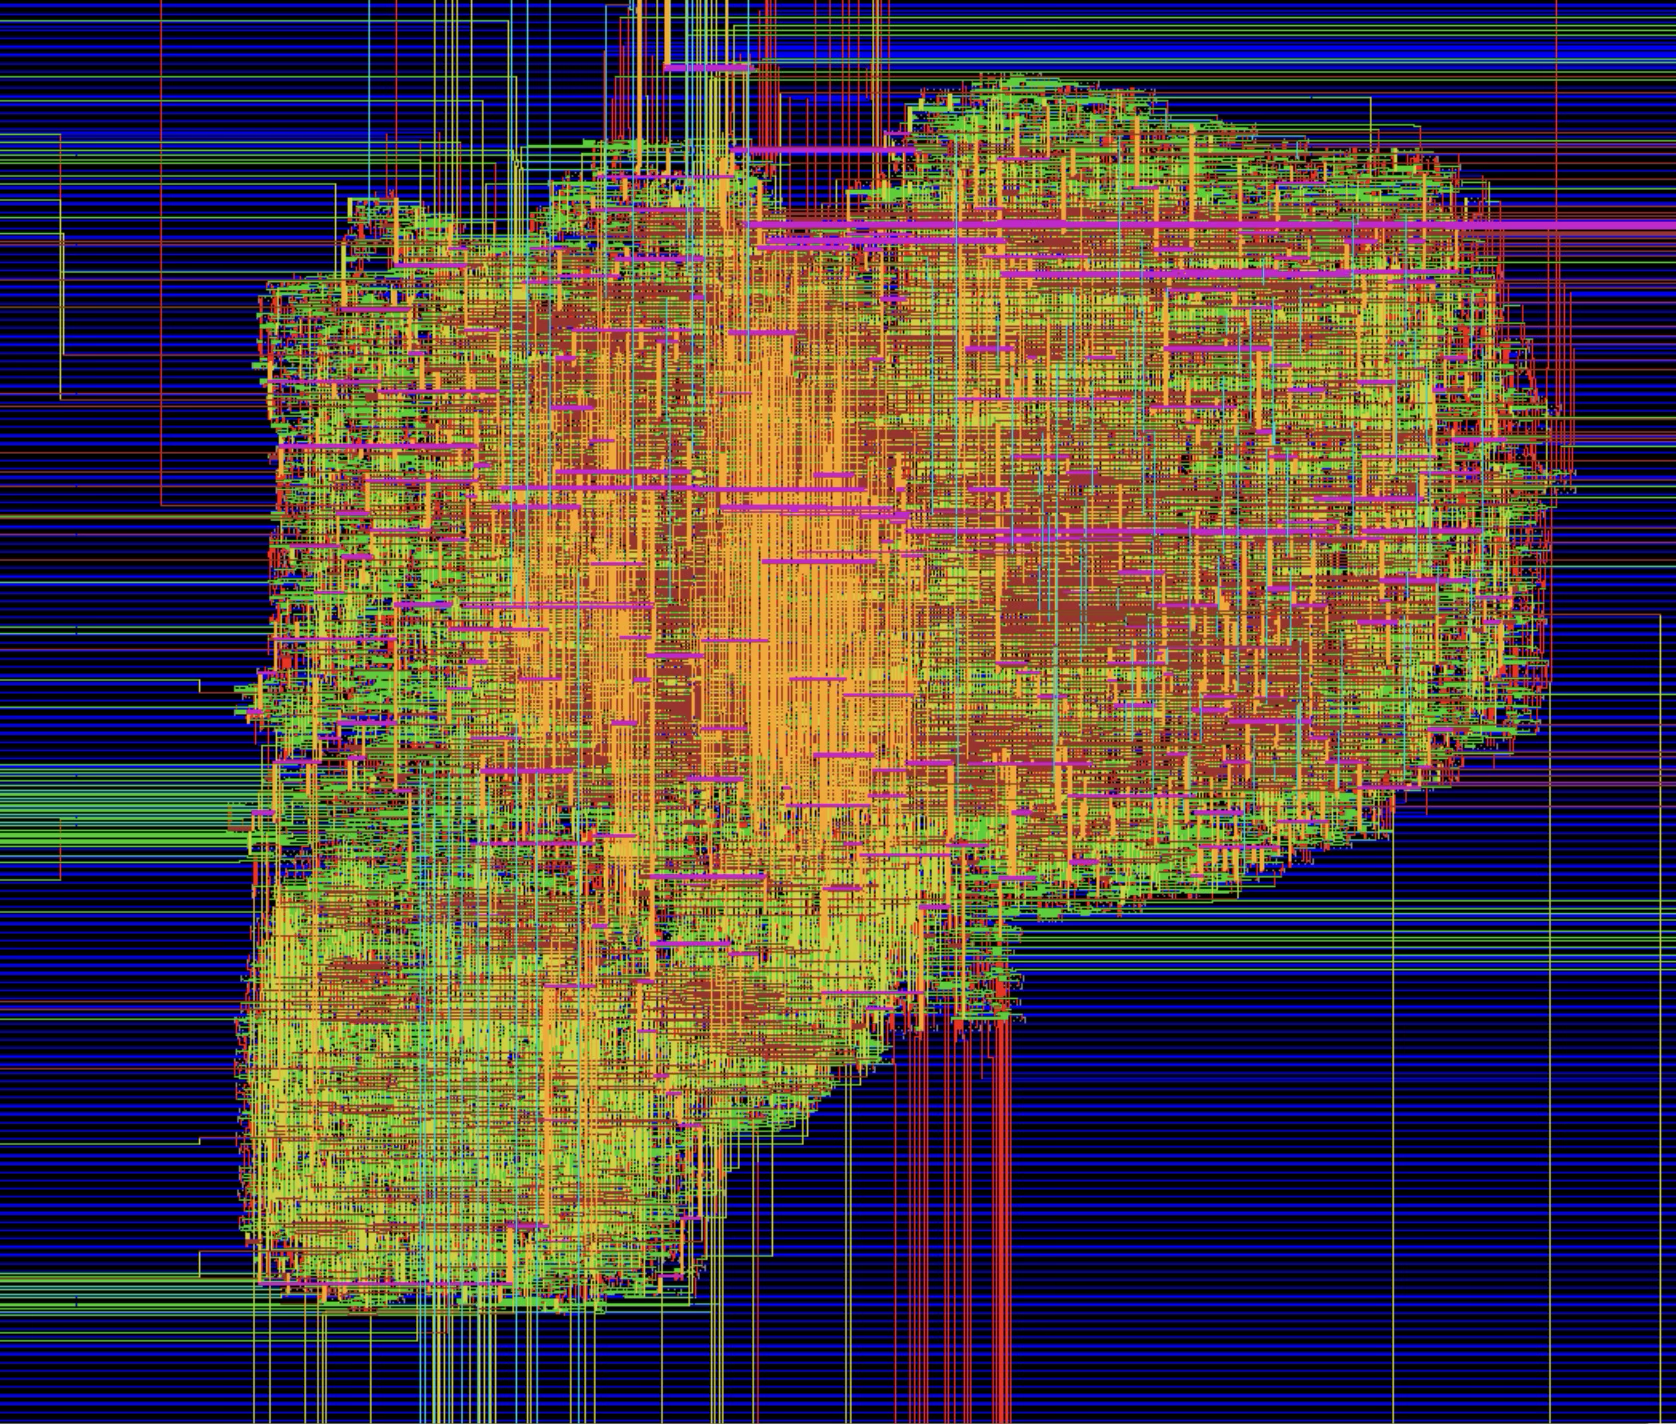
\includegraphics[width=0.8\textwidth]{assets/fig8_2_routing.png}
    \caption{Routed Interconnects}
\end{figure}

Η δεύτερη εικόνα εστιάζει στη δρομολόγηση των σημάτων από τον πυρήνα προς τους ακροδέκτες. Διακρίνονται τα μακριά καλώδια (long interconnects) που απαιτούνται για να συνδέσουν τα ports του μικρού πυρήνα με τα αντίστοιχα I/O cells στην περιφέρεια. Αυτές οι μεγάλες αποστάσεις δρομολόγησης, σε συνδυασμό με την καθυστέρηση των ίδιων των IO cells, εξηγούν τις σημαντικές παραβιάσεις χρονισμού (Setup violations) που παρατηρήθηκαν στα μονοπάτια Inputs-to-Registers (I2R) στον Πίνακα 8.2.

\begin{table}[H]
    \centering
    \caption{Total Area post Routing}
    \begin{tabular}{lr}
        \toprule
        Category & Area ($\mu m^2$) \\
        \midrule
        Άσκηση 1 & 34627.842 \\
        Άσκηση 8 & 7660571.274 \\
        \bottomrule
    \end{tabular}
\end{table}

Η συνολική επιφάνεια του chip εκτοξεύθηκε στα 7.660.571 $\mu m^2$, μια αύξηση της τάξης του $220\times$ σε σύγκριση με τον πυρήνα της Άσκησης 1 (34.627 $\mu m^2$). Αυτό το αποτέλεσμα είναι αναμενόμενο, καθώς τα κελιά εισόδου/εξόδου είναι φυσικά ογκώδη για να υποστηρίξουν τη μηχανική σύνδεση (wire bonding) και να αντέξουν τα ρεύματα οδήγησης, καθιστώντας τον πυρήνα (core) ένα ελάχιστο ποσοστό της συνολικής επιφάνειας του ολοκληρωμένου (Pad Limited Design).

\begin{table}[H]
    \centering
    \caption{Setup and Hold Slack post Routing}
    \begin{tabular}{lrrrr}
        \toprule
         & \multicolumn{2}{c}{\textbf{Άσκηση 1}} & \multicolumn{2}{c}{\textbf{Άσκηση 8}} \\
        \cmidrule(lr){2-3} \cmidrule(lr){4-5}
        Category & Setup Slack (ns) & Hold Slack (ns) & Setup Slack (ns) & Hold Slack (ns) \\
        \midrule
        I2O & - & - & - & - \\
        I2R & 2.531 & 0.241 & -5.880 & 1.760 \\
        R2O & 3.054 & 0.295 & 0.718 & 1.284 \\
        R2R & 1.452 & 0.032 & 1.400 & 0.032 \\
        \bottomrule
    \end{tabular}
\end{table}

Η συνολική κατανάλωση αυξήθηκε από τα 10,46 mW στα 292,3 mW. Όπως αποκαλύπτει ο Πίνακας 8.3, το 95,31\% αυτής της ενέργειας (278,6 mW) καταναλώνεται αποκλειστικά από τα I/Os (κατηγορία “IO”), λόγω των υψηλών τάσεων και των ρευμάτων που απαιτούνται για την οδήγηση των εξωτερικών χωρητικών φορτίων.

\begin{table}[H]
    \centering
    \caption{Power Consumption per Category post Routing}
    \resizebox{\textwidth}{!}{
    \begin{tabular}{lrrrrrrrrrr}
        \toprule
         & \multicolumn{5}{c}{\textbf{Άσκηση 1}} & \multicolumn{5}{c}{\textbf{Άσκηση 8}} \\
        \cmidrule(lr){2-6} \cmidrule(lr){7-11}
        Category & Leakage (mW) & Internal (mW) & Switching (mW) & Total (mW) & Row \% & Leakage (mW) & Internal (mW) & Switching (mW) & Total (mW) & Row \% \\
        \midrule
        Sequential & $1.93\times10^{-3}$ & 3.537 & 0.452 & 3.991 & 38.15 & $1.97\times10^{-3}$ & 3.49 & 1.824 & 5.319 & 1.82 \\
        Combinational & $2.38\times10^{-3}$ & 1.513 & 3.863 & 5.379 & 51.43 & $4.04\times10^{-3}$ & 1.95 & 3.94 & 5.897 & 2.017 \\
        Clock (Comb) & $4.81\times10^{-5}$ & 0.232 & 0.858 & 1.09 & 10.42 & $0.12\times10^{-3}$ & 0.59 & 1.91 & 2.492 & 0.852 \\
        IO & 0 & 0 & 0 & 0 & 0 & 28.86 & 247.1 & 2.68 & 278.6 & 95.31 \\
        Total & $4.355\times10^{-3}$ & 5.283 & 5.173 & 10.46 & 100 & 28.86 & 253.1 & 10.35 & 292.3 & 100 \\
        \bottomrule
    \end{tabular}}
\end{table}

Ενώ τα εσωτερικά μονοπάτια (R2R) διατήρησαν το θετικό τους slack (0,032 ns), παρατηρείται μεγάλη παραβίαση χρονισμού στα μονοπάτια εισόδου (I2R Setup Slack: -5,880 ns). Αυτή η αποτυχία οφείλεται στη σημαντική καθυστέρηση διάδοσης που εισάγουν τα κελιά εισόδου (input pads) σε συνδυασμό με την υψηλή συχνότητα των 250 MHz. Σε μια πραγματική σχεδίαση, αυτό θα απαιτούσε είτε χαλάρωση των περιορισμών χρονισμού για τις εισόδους, είτε χρήση ταχύτερων IO cells, είτε pipeline στα inputs για την αποκατάσταση του χρονισμού.